% This file was created with tikzplotlib v0.10.1.
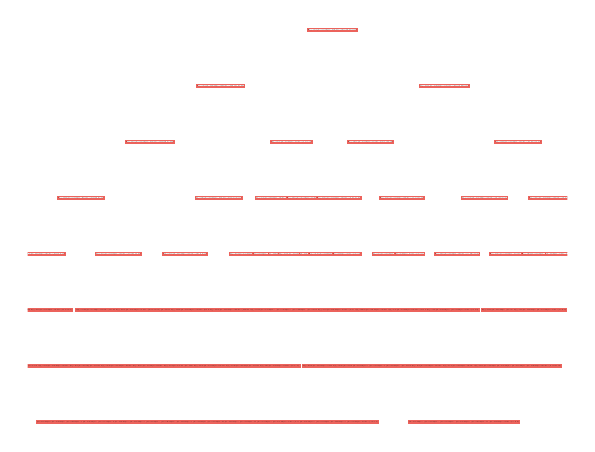
\begin{tikzpicture}

\definecolor{darkgray176}{RGB}{176,176,176}
\definecolor{tomato2369992}{RGB}{236,99,92}

\begin{axis}[
hide x axis,
hide y axis,
tick align=outside,
tick pos=left,
x grid style={darkgray176},
xmin=0, xmax=1,
xtick style={color=black},
y grid style={darkgray176},
ymin=0, ymax=1,
ytick style={color=black}
]
\draw (axis cs:0.0437956204379562,0.0625) node[
  scale=0.05,
  fill=white,
  draw=tomato2369992,
  line width=0.6pt,
  inner sep=3.6pt,
  text=black,
  rotate=0.0,
  align=center
]{gini = 0.273
samples = 78
value = [66, 4, 1, 7]};
\draw (axis cs:0.072992700729927,0.0625) node[
  scale=0.05,
  fill=white,
  draw=tomato2369992,
  line width=0.6pt,
  inner sep=3.6pt,
  text=black,
  rotate=0.0,
  align=center
]{gini = 0.617
samples = 132
value = [71, 16, 9, 36]};
\draw (axis cs:0.102189781021898,0.0625) node[
  scale=0.05,
  fill=white,
  draw=tomato2369992,
  line width=0.6pt,
  inner sep=3.6pt,
  text=black,
  rotate=0.0,
  align=center
]{gini = 0.421
samples = 773
value = [562, 172, 14, 25]};
\draw (axis cs:0.131386861313869,0.0625) node[
  scale=0.05,
  fill=white,
  draw=tomato2369992,
  line width=0.6pt,
  inner sep=3.6pt,
  text=black,
  rotate=0.0,
  align=center
]{gini = 0.588
samples = 275
value = [159, 57, 8, 51]};
\draw (axis cs:0.160583941605839,0.0625) node[
  scale=0.05,
  fill=white,
  draw=tomato2369992,
  line width=0.6pt,
  inner sep=3.6pt,
  text=black,
  rotate=0.0,
  align=center
]{gini = 0.696
samples = 329
value = [39, 63, 85, 142]};
\draw (axis cs:0.18978102189781,0.0625) node[
  scale=0.05,
  fill=white,
  draw=tomato2369992,
  line width=0.6pt,
  inner sep=3.6pt,
  text=black,
  rotate=0.0,
  align=center
]{gini = 0.721
samples = 93
value = [36, 21, 14, 22]};
\draw (axis cs:0.218978102189781,0.0625) node[
  scale=0.05,
  fill=white,
  draw=tomato2369992,
  line width=0.6pt,
  inner sep=3.6pt,
  text=black,
  rotate=0.0,
  align=center
]{gini = 0.564
samples = 245
value = [142, 75, 11, 17]};
\draw (axis cs:0.248175182481752,0.0625) node[
  scale=0.05,
  fill=white,
  draw=tomato2369992,
  line width=0.6pt,
  inner sep=3.6pt,
  text=black,
  rotate=0.0,
  align=center
]{gini = 0.71
samples = 169
value = [63, 36, 18, 52]};
\draw (axis cs:0.277372262773723,0.0625) node[
  scale=0.05,
  fill=white,
  draw=tomato2369992,
  line width=0.6pt,
  inner sep=3.6pt,
  text=black,
  rotate=0.0,
  align=center
]{gini = 0.406
samples = 1384
value = [996, 4, 2, 382]};
\draw (axis cs:0.306569343065693,0.0625) node[
  scale=0.05,
  fill=white,
  draw=tomato2369992,
  line width=0.6pt,
  inner sep=3.6pt,
  text=black,
  rotate=0.0,
  align=center
]{gini = 0.252
samples = 1506
value = [1285, 6, 4, 211]};
\draw (axis cs:0.335766423357664,0.0625) node[
  scale=0.05,
  fill=white,
  draw=tomato2369992,
  line width=0.6pt,
  inner sep=3.6pt,
  text=black,
  rotate=0.0,
  align=center
]{gini = 0.281
samples = 679
value = [571, 63, 5, 40]};
\draw (axis cs:0.364963503649635,0.0625) node[
  scale=0.05,
  fill=white,
  draw=tomato2369992,
  line width=0.6pt,
  inner sep=3.6pt,
  text=black,
  rotate=0.0,
  align=center
]{gini = 0.657
samples = 1053
value = [508, 71, 189, 285]};
\draw (axis cs:0.394160583941606,0.0625) node[
  scale=0.05,
  fill=white,
  draw=tomato2369992,
  line width=0.6pt,
  inner sep=3.6pt,
  text=black,
  rotate=0.0,
  align=center
]{gini = 0.257
samples = 546
value = [467, 54, 0, 25]};
\draw (axis cs:0.423357664233577,0.0625) node[
  scale=0.05,
  fill=white,
  draw=tomato2369992,
  line width=0.6pt,
  inner sep=3.6pt,
  text=black,
  rotate=0.0,
  align=center
]{gini = 0.51
samples = 723
value = [478, 56, 36, 153]};
\draw (axis cs:0.452554744525547,0.0625) node[
  scale=0.05,
  fill=white,
  draw=tomato2369992,
  line width=0.6pt,
  inner sep=3.6pt,
  text=black,
  rotate=0.0,
  align=center
]{gini = 0.567
samples = 66
value = [2, 20, 6, 38]};
\draw (axis cs:0.481751824817518,0.0625) node[
  scale=0.05,
  fill=white,
  draw=tomato2369992,
  line width=0.6pt,
  inner sep=3.6pt,
  text=black,
  rotate=0.0,
  align=center
]{gini = 0.596
samples = 68
value = [29, 31, 0, 8]};
\draw (axis cs:0.532846715328467,0.0625) node[
  scale=0.05,
  fill=white,
  draw=tomato2369992,
  line width=0.6pt,
  inner sep=3.6pt,
  text=black,
  rotate=0.0,
  align=center
]{gini = 0.137
samples = 332
value = [4, 308, 17, 3]};
\draw (axis cs:0.562043795620438,0.0625) node[
  scale=0.05,
  fill=white,
  draw=tomato2369992,
  line width=0.6pt,
  inner sep=3.6pt,
  text=black,
  rotate=0.0,
  align=center
]{gini = 0.568
samples = 32
value = [0, 17, 12, 3]};
\draw (axis cs:0.591240875912409,0.0625) node[
  scale=0.05,
  fill=white,
  draw=tomato2369992,
  line width=0.6pt,
  inner sep=3.6pt,
  text=black,
  rotate=0.0,
  align=center
]{gini = 0.422
samples = 376
value = [10, 278, 59, 29]};
\draw (axis cs:0.62043795620438,0.0625) node[
  scale=0.05,
  fill=white,
  draw=tomato2369992,
  line width=0.6pt,
  inner sep=3.6pt,
  text=black,
  rotate=0.0,
  align=center
]{gini = 0.629
samples = 135
value = [6, 50, 63, 16]};
\draw (axis cs:0.737226277372263,0.0625) node[
  scale=0.05,
  fill=white,
  draw=tomato2369992,
  line width=0.6pt,
  inner sep=3.6pt,
  text=black,
  rotate=0.0,
  align=center
]{gini = 0.695
samples = 903
value = [293, 338, 213, 59]};
\draw (axis cs:0.766423357664234,0.0625) node[
  scale=0.05,
  fill=white,
  draw=tomato2369992,
  line width=0.6pt,
  inner sep=3.6pt,
  text=black,
  rotate=0.0,
  align=center
]{gini = 0.651
samples = 746
value = [145, 372, 180, 49]};
\draw (axis cs:0.795620437956204,0.0625) node[
  scale=0.05,
  fill=white,
  draw=tomato2369992,
  line width=0.6pt,
  inner sep=3.6pt,
  text=black,
  rotate=0.0,
  align=center
]{gini = 0.689
samples = 347
value = [13, 105, 117, 112]};
\draw (axis cs:0.824817518248175,0.0625) node[
  scale=0.05,
  fill=white,
  draw=tomato2369992,
  line width=0.6pt,
  inner sep=3.6pt,
  text=black,
  rotate=0.0,
  align=center
]{gini = 0.713
samples = 464
value = [115, 185, 104, 60]};
\draw (axis cs:0.854014598540146,0.0625) node[
  scale=0.05,
  fill=white,
  draw=tomato2369992,
  line width=0.6pt,
  inner sep=3.6pt,
  text=black,
  rotate=0.0,
  align=center
]{gini = 0.249
samples = 2390
value = [33, 2058, 208, 91]};
\draw (axis cs:0.883211678832117,0.0625) node[
  scale=0.05,
  fill=white,
  draw=tomato2369992,
  line width=0.6pt,
  inner sep=3.6pt,
  text=black,
  rotate=0.0,
  align=center
]{gini = 0.602
samples = 34
value = [0, 6, 18, 10]};
\draw (axis cs:0.0291970802919708,0.1875) node[
  scale=0.05,
  fill=white,
  draw=tomato2369992,
  line width=0.6pt,
  inner sep=3.6pt,
  text=black,
  rotate=0.0,
  align=center
]{gini = 0.657
samples = 111
value = [38, 9, 14, 50]};
\draw (axis cs:0.0583941605839416,0.1875) node[
  scale=0.05,
  fill=white,
  draw=tomato2369992,
  line width=0.6pt,
  inner sep=3.6pt,
  text=black,
  rotate=0.0,
  align=center
]{X[2] <= 281.18
gini = 0.521
samples = 210
value = [137, 20, 10, 43]};
\draw (axis cs:0.116788321167883,0.1875) node[
  scale=0.05,
  fill=white,
  draw=tomato2369992,
  line width=0.6pt,
  inner sep=3.6pt,
  text=black,
  rotate=0.0,
  align=center
]{X[2] <= 24.87
gini = 0.473
samples = 1048
value = [721, 229, 22, 76]};
\draw (axis cs:0.145985401459854,0.1875) node[
  scale=0.05,
  fill=white,
  draw=tomato2369992,
  line width=0.6pt,
  inner sep=3.6pt,
  text=black,
  rotate=0.0,
  align=center
]{gini = 0.586
samples = 1344
value = [632, 581, 39, 92]};
\draw (axis cs:0.175182481751825,0.1875) node[
  scale=0.05,
  fill=white,
  draw=tomato2369992,
  line width=0.6pt,
  inner sep=3.6pt,
  text=black,
  rotate=0.0,
  align=center
]{X[2] <= 677.505
gini = 0.723
samples = 422
value = [75, 84, 99, 164]};
\draw (axis cs:0.233576642335766,0.1875) node[
  scale=0.05,
  fill=white,
  draw=tomato2369992,
  line width=0.6pt,
  inner sep=3.6pt,
  text=black,
  rotate=0.0,
  align=center
]{X[2] <= 481.365
gini = 0.65
samples = 414
value = [205, 111, 29, 69]};
\draw (axis cs:0.291970802919708,0.1875) node[
  scale=0.05,
  fill=white,
  draw=tomato2369992,
  line width=0.6pt,
  inner sep=3.6pt,
  text=black,
  rotate=0.0,
  align=center
]{X[2] <= 463.94
gini = 0.335
samples = 2890
value = [2281, 10, 6, 593]};
\draw (axis cs:0.321167883211679,0.1875) node[
  scale=0.05,
  fill=white,
  draw=tomato2369992,
  line width=0.6pt,
  inner sep=3.6pt,
  text=black,
  rotate=0.0,
  align=center
]{gini = 0.207
samples = 2613
value = [2308, 8, 4, 293]};
\draw (axis cs:0.35036496350365,0.1875) node[
  scale=0.05,
  fill=white,
  draw=tomato2369992,
  line width=0.6pt,
  inner sep=3.6pt,
  text=black,
  rotate=0.0,
  align=center
]{X[2] <= 158.585
gini = 0.558
samples = 1732
value = [1079, 134, 194, 325]};
\draw (axis cs:0.408759124087591,0.1875) node[
  scale=0.05,
  fill=white,
  draw=tomato2369992,
  line width=0.6pt,
  inner sep=3.6pt,
  text=black,
  rotate=0.0,
  align=center
]{X[2] <= 368.045
gini = 0.417
samples = 1269
value = [945, 110, 36, 178]};
\draw (axis cs:0.437956204379562,0.1875) node[
  scale=0.05,
  fill=white,
  draw=tomato2369992,
  line width=0.6pt,
  inner sep=3.6pt,
  text=black,
  rotate=0.0,
  align=center
]{gini = 0.593
samples = 177
value = [82, 76, 4, 15]};
\draw (axis cs:0.467153284671533,0.1875) node[
  scale=0.05,
  fill=white,
  draw=tomato2369992,
  line width=0.6pt,
  inner sep=3.6pt,
  text=black,
  rotate=0.0,
  align=center
]{X[3] <= 124.2
gini = 0.682
samples = 134
value = [31, 51, 6, 46]};
\draw (axis cs:0.547445255474453,0.1875) node[
  scale=0.05,
  fill=white,
  draw=tomato2369992,
  line width=0.6pt,
  inner sep=3.6pt,
  text=black,
  rotate=0.0,
  align=center
]{X[2] <= 217.185
gini = 0.196
samples = 364
value = [4, 325, 29, 6]};
\draw (axis cs:0.605839416058394,0.1875) node[
  scale=0.05,
  fill=white,
  draw=tomato2369992,
  line width=0.6pt,
  inner sep=3.6pt,
  text=black,
  rotate=0.0,
  align=center
]{X[1] <= 752.075
gini = 0.522
samples = 511
value = [16, 328, 122, 45]};
\draw (axis cs:0.635036496350365,0.1875) node[
  scale=0.05,
  fill=white,
  draw=tomato2369992,
  line width=0.6pt,
  inner sep=3.6pt,
  text=black,
  rotate=0.0,
  align=center
]{gini = 0.257
samples = 2909
value = [212, 23, 2492, 182]};
\draw (axis cs:0.664233576642336,0.1875) node[
  scale=0.05,
  fill=white,
  draw=tomato2369992,
  line width=0.6pt,
  inner sep=3.6pt,
  text=black,
  rotate=0.0,
  align=center
]{gini = 0.163
samples = 3639
value = [87, 1, 3320, 231]};
\draw (axis cs:0.693430656934307,0.1875) node[
  scale=0.05,
  fill=white,
  draw=tomato2369992,
  line width=0.6pt,
  inner sep=3.6pt,
  text=black,
  rotate=0.0,
  align=center
]{gini = 0.277
samples = 960
value = [50, 7, 809, 94]};
\draw (axis cs:0.722627737226277,0.1875) node[
  scale=0.05,
  fill=white,
  draw=tomato2369992,
  line width=0.6pt,
  inner sep=3.6pt,
  text=black,
  rotate=0.0,
  align=center
]{gini = 0.396
samples = 768
value = [40, 7, 578, 143]};
\draw (axis cs:0.751824817518248,0.1875) node[
  scale=0.05,
  fill=white,
  draw=tomato2369992,
  line width=0.6pt,
  inner sep=3.6pt,
  text=black,
  rotate=0.0,
  align=center
]{X[1] <= 493.4
gini = 0.683
samples = 1649
value = [438, 710, 393, 108]};
\draw (axis cs:0.81021897810219,0.1875) node[
  scale=0.05,
  fill=white,
  draw=tomato2369992,
  line width=0.6pt,
  inner sep=3.6pt,
  text=black,
  rotate=0.0,
  align=center
]{X[3] <= 193.36
gini = 0.728
samples = 811
value = [128, 290, 221, 172]};
\draw (axis cs:0.868613138686131,0.1875) node[
  scale=0.05,
  fill=white,
  draw=tomato2369992,
  line width=0.6pt,
  inner sep=3.6pt,
  text=black,
  rotate=0.0,
  align=center
]{X[2] <= 403.61
gini = 0.264
samples = 2424
value = [33, 2064, 226, 101]};
\draw (axis cs:0.897810218978102,0.1875) node[
  scale=0.05,
  fill=white,
  draw=tomato2369992,
  line width=0.6pt,
  inner sep=3.6pt,
  text=black,
  rotate=0.0,
  align=center
]{gini = 0.625
samples = 137
value = [5, 68, 45, 19]};
\draw (axis cs:0.927007299270073,0.1875) node[
  scale=0.05,
  fill=white,
  draw=tomato2369992,
  line width=0.6pt,
  inner sep=3.6pt,
  text=black,
  rotate=0.0,
  align=center
]{gini = 0.166
samples = 746
value = [23, 11, 680, 32]};
\draw (axis cs:0.956204379562044,0.1875) node[
  scale=0.05,
  fill=white,
  draw=tomato2369992,
  line width=0.6pt,
  inner sep=3.6pt,
  text=black,
  rotate=0.0,
  align=center
]{gini = 0.342
samples = 1343
value = [91, 34, 1076, 142]};
\draw (axis cs:0.0145985401459854,0.3125) node[
  scale=0.05,
  fill=white,
  draw=tomato2369992,
  line width=0.6pt,
  inner sep=3.6pt,
  text=black,
  rotate=0.0,
  align=center
]{gini = 0.08
samples = 924
value = [886, 15, 0, 23]};
\draw (axis cs:0.0437956204379562,0.3125) node[
  scale=0.05,
  fill=white,
  draw=tomato2369992,
  line width=0.6pt,
  inner sep=3.6pt,
  text=black,
  rotate=0.0,
  align=center
]{X[3] <= 48.53
gini = 0.605
samples = 321
value = [175, 29, 24, 93]};
\draw (axis cs:0.131386861313869,0.3125) node[
  scale=0.05,
  fill=white,
  draw=tomato2369992,
  line width=0.6pt,
  inner sep=3.6pt,
  text=black,
  rotate=0.0,
  align=center
]{X[1] <= 253.105
gini = 0.56
samples = 2392
value = [1353, 810, 61, 168]};
\draw (axis cs:0.204379562043796,0.3125) node[
  scale=0.05,
  fill=white,
  draw=tomato2369992,
  line width=0.6pt,
  inner sep=3.6pt,
  text=black,
  rotate=0.0,
  align=center
]{X[3] <= 228.775
gini = 0.732
samples = 836
value = [280, 195, 128, 233]};
\draw (axis cs:0.277372262773723,0.3125) node[
  scale=0.05,
  fill=white,
  draw=tomato2369992,
  line width=0.6pt,
  inner sep=3.6pt,
  text=black,
  rotate=0.0,
  align=center
]{gini = 0.053
samples = 4002
value = [3894, 3, 0, 105]};
\draw (axis cs:0.306569343065693,0.3125) node[
  scale=0.05,
  fill=white,
  draw=tomato2369992,
  line width=0.6pt,
  inner sep=3.6pt,
  text=black,
  rotate=0.0,
  align=center
]{X[3] <= 125.485
gini = 0.279
samples = 5503
value = [4589, 18, 10, 886]};
\draw (axis cs:0.37956204379562,0.3125) node[
  scale=0.05,
  fill=white,
  draw=tomato2369992,
  line width=0.6pt,
  inner sep=3.6pt,
  text=black,
  rotate=0.0,
  align=center
]{X[3] <= 162.395
gini = 0.505
samples = 3001
value = [2024, 244, 230, 503]};
\draw (axis cs:0.452554744525547,0.3125) node[
  scale=0.05,
  fill=white,
  draw=tomato2369992,
  line width=0.6pt,
  inner sep=3.6pt,
  text=black,
  rotate=0.0,
  align=center
]{X[2] <= 127.135
gini = 0.662
samples = 311
value = [113, 127, 10, 61]};
\draw (axis cs:0.489051094890511,0.3125) node[
  scale=0.05,
  fill=white,
  draw=tomato2369992,
  line width=0.6pt,
  inner sep=3.6pt,
  text=black,
  rotate=0.0,
  align=center
]{gini = 0.638
samples = 69
value = [19, 11, 4, 35]};
\draw (axis cs:0.518248175182482,0.3125) node[
  scale=0.05,
  fill=white,
  draw=tomato2369992,
  line width=0.6pt,
  inner sep=3.6pt,
  text=black,
  rotate=0.0,
  align=center
]{gini = 0.104
samples = 127
value = [7, 0, 0, 120]};
\draw (axis cs:0.547445255474453,0.3125) node[
  scale=0.05,
  fill=white,
  draw=tomato2369992,
  line width=0.6pt,
  inner sep=3.6pt,
  text=black,
  rotate=0.0,
  align=center
]{gini = 0.725
samples = 228
value = [51, 75, 72, 30]};
\draw (axis cs:0.576642335766423,0.3125) node[
  scale=0.05,
  fill=white,
  draw=tomato2369992,
  line width=0.6pt,
  inner sep=3.6pt,
  text=black,
  rotate=0.0,
  align=center
]{X[3] <= 57.895
gini = 0.409
samples = 875
value = [20, 653, 151, 51]};
\draw (axis cs:0.64963503649635,0.3125) node[
  scale=0.05,
  fill=white,
  draw=tomato2369992,
  line width=0.6pt,
  inner sep=3.6pt,
  text=black,
  rotate=0.0,
  align=center
]{X[1] <= 1024.315
gini = 0.206
samples = 6548
value = [299, 24, 5812, 413]};
\draw (axis cs:0.708029197080292,0.3125) node[
  scale=0.05,
  fill=white,
  draw=tomato2369992,
  line width=0.6pt,
  inner sep=3.6pt,
  text=black,
  rotate=0.0,
  align=center
]{X[2] <= 0.935
gini = 0.334
samples = 1728
value = [90, 14, 1387, 237]};
\draw (axis cs:0.781021897810219,0.3125) node[
  scale=0.05,
  fill=white,
  draw=tomato2369992,
  line width=0.6pt,
  inner sep=3.6pt,
  text=black,
  rotate=0.0,
  align=center
]{X[2] <= 63.475
gini = 0.707
samples = 2460
value = [566, 1000, 614, 280]};
\draw (axis cs:0.81021897810219,0.3125) node[
  scale=0.05,
  fill=white,
  draw=tomato2369992,
  line width=0.6pt,
  inner sep=3.6pt,
  text=black,
  rotate=0.0,
  align=center
]{gini = 0.0
samples = 28
value = [0, 0, 0, 28]};
\draw (axis cs:0.883211678832117,0.3125) node[
  scale=0.05,
  fill=white,
  draw=tomato2369992,
  line width=0.6pt,
  inner sep=3.6pt,
  text=black,
  rotate=0.0,
  align=center
]{X[1] <= 769.135
gini = 0.293
samples = 2561
value = [38, 2132, 271, 120]};
\draw (axis cs:0.912408759124088,0.3125) node[
  scale=0.05,
  fill=white,
  draw=tomato2369992,
  line width=0.6pt,
  inner sep=3.6pt,
  text=black,
  rotate=0.0,
  align=center
]{gini = 0.0
samples = 78
value = [0, 0, 0, 78]};
\draw (axis cs:0.941605839416058,0.3125) node[
  scale=0.05,
  fill=white,
  draw=tomato2369992,
  line width=0.6pt,
  inner sep=3.6pt,
  text=black,
  rotate=0.0,
  align=center
]{X[3] <= 37.64
gini = 0.283
samples = 2089
value = [114, 45, 1756, 174]};
\draw (axis cs:0.970802919708029,0.3125) node[
  scale=0.05,
  fill=white,
  draw=tomato2369992,
  line width=0.6pt,
  inner sep=3.6pt,
  text=black,
  rotate=0.0,
  align=center
]{gini = 0.565
samples = 61
value = [4, 2, 34, 21]};
\draw (axis cs:0.0291970802919708,0.4375) node[
  scale=0.05,
  fill=white,
  draw=tomato2369992,
  line width=0.6pt,
  inner sep=3.6pt,
  text=black,
  rotate=0.0,
  align=center
]{X[2] <= 36.76
gini = 0.263
samples = 1245
value = [1061, 44, 24, 116]};
\draw (axis cs:0.167883211678832,0.4375) node[
  scale=0.05,
  fill=white,
  draw=tomato2369992,
  line width=0.6pt,
  inner sep=3.6pt,
  text=black,
  rotate=0.0,
  align=center
]{X[2] <= 229.5
gini = 0.628
samples = 3228
value = [1633, 1005, 189, 401]};
\draw (axis cs:0.291970802919708,0.4375) node[
  scale=0.05,
  fill=white,
  draw=tomato2369992,
  line width=0.6pt,
  inner sep=3.6pt,
  text=black,
  rotate=0.0,
  align=center
]{X[2] <= 50.855
gini = 0.193
samples = 9505
value = [8483, 21, 10, 991]};
\draw (axis cs:0.416058394160584,0.4375) node[
  scale=0.05,
  fill=white,
  draw=tomato2369992,
  line width=0.6pt,
  inner sep=3.6pt,
  text=black,
  rotate=0.0,
  align=center
]{X[1] <= 218.34
gini = 0.537
samples = 3312
value = [2137, 371, 240, 564]};
\draw (axis cs:0.445255474452555,0.4375) node[
  scale=0.05,
  fill=white,
  draw=tomato2369992,
  line width=0.6pt,
  inner sep=3.6pt,
  text=black,
  rotate=0.0,
  align=center
]{gini = 0.618
samples = 58
value = [29, 9, 1, 19]};
\draw (axis cs:0.474452554744526,0.4375) node[
  scale=0.05,
  fill=white,
  draw=tomato2369992,
  line width=0.6pt,
  inner sep=3.6pt,
  text=black,
  rotate=0.0,
  align=center
]{gini = 0.445
samples = 122
value = [32, 2, 3, 85]};
\draw (axis cs:0.503649635036496,0.4375) node[
  scale=0.05,
  fill=white,
  draw=tomato2369992,
  line width=0.6pt,
  inner sep=3.6pt,
  text=black,
  rotate=0.0,
  align=center
]{X[0] <= 289.485
gini = 0.353
samples = 196
value = [26, 11, 4, 155]};
\draw (axis cs:0.532846715328467,0.4375) node[
  scale=0.05,
  fill=white,
  draw=tomato2369992,
  line width=0.6pt,
  inner sep=3.6pt,
  text=black,
  rotate=0.0,
  align=center
]{gini = 0.051
samples = 381
value = [10, 0, 0, 371]};
\draw (axis cs:0.562043795620438,0.4375) node[
  scale=0.05,
  fill=white,
  draw=tomato2369992,
  line width=0.6pt,
  inner sep=3.6pt,
  text=black,
  rotate=0.0,
  align=center
]{X[1] <= 572.465
gini = 0.514
samples = 1103
value = [71, 728, 223, 81]};
\draw (axis cs:0.591240875912409,0.4375) node[
  scale=0.05,
  fill=white,
  draw=tomato2369992,
  line width=0.6pt,
  inner sep=3.6pt,
  text=black,
  rotate=0.0,
  align=center
]{gini = 0.0
samples = 34
value = [0, 0, 0, 34]};
\draw (axis cs:0.678832116788321,0.4375) node[
  scale=0.05,
  fill=white,
  draw=tomato2369992,
  line width=0.6pt,
  inner sep=3.6pt,
  text=black,
  rotate=0.0,
  align=center
]{X[5] <= 52.5
gini = 0.235
samples = 8276
value = [389, 38, 7199, 650]};
\draw (axis cs:0.708029197080292,0.4375) node[
  scale=0.05,
  fill=white,
  draw=tomato2369992,
  line width=0.6pt,
  inner sep=3.6pt,
  text=black,
  rotate=0.0,
  align=center
]{gini = 0.0
samples = 155
value = [0, 0, 0, 155]};
\draw (axis cs:0.795620437956204,0.4375) node[
  scale=0.05,
  fill=white,
  draw=tomato2369992,
  line width=0.6pt,
  inner sep=3.6pt,
  text=black,
  rotate=0.0,
  align=center
]{X[5] <= 2502.5
gini = 0.71
samples = 2488
value = [566, 1000, 614, 308]};
\draw (axis cs:0.897810218978102,0.4375) node[
  scale=0.05,
  fill=white,
  draw=tomato2369992,
  line width=0.6pt,
  inner sep=3.6pt,
  text=black,
  rotate=0.0,
  align=center
]{X[5] <= 2502.5
gini = 0.331
samples = 2639
value = [38, 2132, 271, 198]};
\draw (axis cs:0.956204379562044,0.4375) node[
  scale=0.05,
  fill=white,
  draw=tomato2369992,
  line width=0.6pt,
  inner sep=3.6pt,
  text=black,
  rotate=0.0,
  align=center
]{X[5] <= 210.0
gini = 0.295
samples = 2150
value = [118, 47, 1790, 195]};
\draw (axis cs:0.985401459854015,0.4375) node[
  scale=0.05,
  fill=white,
  draw=tomato2369992,
  line width=0.6pt,
  inner sep=3.6pt,
  text=black,
  rotate=0.0,
  align=center
]{gini = 0.0
samples = 52
value = [0, 0, 0, 52]};
\draw (axis cs:0.0985401459854015,0.5625) node[
  scale=0.05,
  fill=white,
  draw=tomato2369992,
  line width=0.6pt,
  inner sep=3.6pt,
  text=black,
  rotate=0.0,
  align=center
]{X[1] <= 130.07
gini = 0.567
samples = 4473
value = [2694, 1049, 213, 517]};
\draw (axis cs:0.354014598540146,0.5625) node[
  scale=0.05,
  fill=white,
  draw=tomato2369992,
  line width=0.6pt,
  inner sep=3.6pt,
  text=black,
  rotate=0.0,
  align=center
]{X[1] <= 0.005
gini = 0.297
samples = 12817
value = [10620, 392, 250, 1555]};
\draw (axis cs:0.45985401459854,0.5625) node[
  scale=0.05,
  fill=white,
  draw=tomato2369992,
  line width=0.6pt,
  inner sep=3.6pt,
  text=black,
  rotate=0.0,
  align=center
]{X[2] <= 57.92
gini = 0.547
samples = 180
value = [61, 11, 4, 104]};
\draw (axis cs:0.518248175182482,0.5625) node[
  scale=0.05,
  fill=white,
  draw=tomato2369992,
  line width=0.6pt,
  inner sep=3.6pt,
  text=black,
  rotate=0.0,
  align=center
]{X[5] <= 2502.5
gini = 0.165
samples = 577
value = [36, 11, 4, 526]};
\draw (axis cs:0.576642335766423,0.5625) node[
  scale=0.05,
  fill=white,
  draw=tomato2369992,
  line width=0.6pt,
  inner sep=3.6pt,
  text=black,
  rotate=0.0,
  align=center
]{X[5] <= 2502.5
gini = 0.537
samples = 1137
value = [71, 728, 223, 115]};
\draw (axis cs:0.693430656934307,0.5625) node[
  scale=0.05,
  fill=white,
  draw=tomato2369992,
  line width=0.6pt,
  inner sep=3.6pt,
  text=black,
  rotate=0.0,
  align=center
]{X[5] <= 2502.5
gini = 0.26
samples = 8431
value = [389, 38, 7199, 805]};
\draw (axis cs:0.846715328467153,0.5625) node[
  scale=0.05,
  fill=white,
  draw=tomato2369992,
  line width=0.6pt,
  inner sep=3.6pt,
  text=black,
  rotate=0.0,
  align=center
]{X[1] <= 563.315
gini = 0.573
samples = 5127
value = [604, 3132, 885, 506]};
\draw (axis cs:0.970802919708029,0.5625) node[
  scale=0.05,
  fill=white,
  draw=tomato2369992,
  line width=0.6pt,
  inner sep=3.6pt,
  text=black,
  rotate=0.0,
  align=center
]{X[5] <= 2502.5
gini = 0.323
samples = 2202
value = [118, 47, 1790, 247]};
\draw (axis cs:0.226277372262774,0.6875) node[
  scale=0.05,
  fill=white,
  draw=tomato2369992,
  line width=0.6pt,
  inner sep=3.6pt,
  text=black,
  rotate=0.0,
  align=center
]{X[0] <= 285.76
gini = 0.385
samples = 17290
value = [13314, 1441, 463, 2072]};
\draw (axis cs:0.489051094890511,0.6875) node[
  scale=0.05,
  fill=white,
  draw=tomato2369992,
  line width=0.6pt,
  inner sep=3.6pt,
  text=black,
  rotate=0.0,
  align=center
]{X[5] <= 1067.5
gini = 0.29
samples = 757
value = [97, 22, 8, 630]};
\draw (axis cs:0.635036496350365,0.6875) node[
  scale=0.05,
  fill=white,
  draw=tomato2369992,
  line width=0.6pt,
  inner sep=3.6pt,
  text=black,
  rotate=0.0,
  align=center
]{X[1] <= 784.155
gini = 0.38
samples = 9568
value = [460, 766, 7422, 920]};
\draw (axis cs:0.908759124087591,0.6875) node[
  scale=0.05,
  fill=white,
  draw=tomato2369992,
  line width=0.6pt,
  inner sep=3.6pt,
  text=black,
  rotate=0.0,
  align=center
]{X[1] <= 782.03
gini = 0.658
samples = 7329
value = [722, 3179, 2675, 753]};
\draw (axis cs:0.357664233576642,0.8125) node[
  scale=0.05,
  fill=white,
  draw=tomato2369992,
  line width=0.6pt,
  inner sep=3.6pt,
  text=black,
  rotate=0.0,
  align=center
]{X[5] <= 525.0
gini = 0.418
samples = 18047
value = [13411, 1463, 471, 2702]};
\draw (axis cs:0.771897810218978,0.8125) node[
  scale=0.05,
  fill=white,
  draw=tomato2369992,
  line width=0.6pt,
  inner sep=3.6pt,
  text=black,
  rotate=0.0,
  align=center
]{X[0] <= 277.225
gini = 0.574
samples = 16897
value = [1182, 3945, 10097, 1673]};
\draw (axis cs:0.56478102189781,0.9375) node[
  scale=0.05,
  fill=white,
  draw=tomato2369992,
  line width=0.6pt,
  inner sep=3.6pt,
  text=black,
  rotate=0.0,
  align=center
]{X[1] <= 385.71
gini = 0.695
samples = 34944
value = [14593, 5408, 10568, 4375]};
\end{axis}

\end{tikzpicture}
